\begin{SCfigure*}
	\centering
	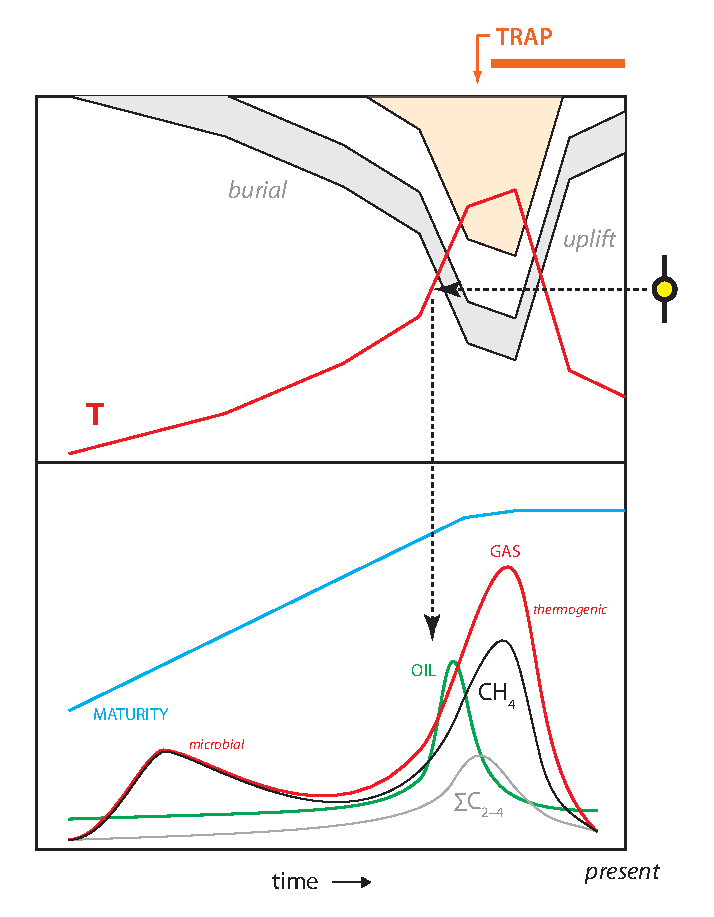
\includegraphics[width=0.6\textwidth]{figures/Fig1.9.pdf}
	\captionsetup{format=myformat}	% hrule beneath caption
	\caption[Petroleum system applications of
	\textsuperscript{13}CH\textsubscript{3}D]{Petroleum system applications of
		\textsuperscript{13}CH\textsubscript{3}D. The potential application
		space of methane isotopologue geothermometry and geospeedometry include
		the ability to link key hydrocarbon system elements (particularly
		elements of source, charge, and trap) in time and space, to calibrate
		and/or validate basin model predictions and coupled source rock
		maturation simulations, and to define a new metric of maturity based
		solely on fluid chemistry.}
	\label{fig:1:9}
\end{SCfigure*}